\chapter{A Critique of the Master Sintering Curve Analysis of Sintering Processes}

\section{Introduction}
The master sintering curve (MSC) approach was developed by Su and Johnson \cite{Su1996} to generalize the densification profile of a sintering powder with a single curve for the entire sintering time/temperature. The MSC approach is based on a combined-stage sintering model developed by Hansen et al, \cite{Hansen1992} given as:

%%
\begin{equation}
\label{Ch6-eq: eq1}
\frac{1}{\rho} \frac{d\rho}{dt} = \frac{3 \gamma \Omega}{k_{B}T} \left( \frac{\delta D_{b} \Gamma_{b}}{G^{4}} + \frac{D_{v} \Gamma_{v}}{G^{3}} \right)
\end{equation}
%%

\noindent where $\rho$ is relative density of the powder compact, $d\rho/dt$ is densification rate, $\gamma$ is surface energy, $\Omega$ is molar volume, $k_{B}$ is Boltzmann's constant, $T$ is absolute temperature, $G$ is grain size, $D$ is diffusion coefficient, $\delta$ is grain boundary thickness, and $\Gamma$ is a geometric scaling factor. The subscripts $b$ and $v$ represent grain boundary and volume diffusion mechanisms, respectively. The MSC is derived by simplifying the combined-stage sintering model (Eq. \ref{Ch6-eq: eq1}) to account for only a single diffusion mechanism, and by considering diffusion as thermally-activated via an activation energy $Q$. The resulting equation is given as:

%%
\begin{equation}
\label{Ch6-eq: eq2}
\frac{1}{\rho} \frac{d\rho}{dt} = \frac{3 \gamma \Omega}{k_{B}T} \left( \frac{D \Gamma}{G^{n}} \right)
\end{equation}
%%

\noindent where

%%
\begin{equation}
\label{Ch6-eq: eq3}
D = D_{0}e^{-Q/RT}
\end{equation}
%%

\noindent and $R$ is the ideal gas constant. Eq. \ref{Ch6-eq: eq2} is re-written to collect microstructural parameters on the left hand side and temperature dependent parameters on the right hand side:

%%
\begin{equation}
\label{Ch6-eq: eq4}
\frac{k_{B} G^{n}}{3 \rho \gamma \Omega \Gamma D_{0}} \frac{d\rho}{dt} = \frac{1}{T} exp \left( -\frac{Q}{RT} \right) = \frac{d \Theta}{dt}
\end{equation}
%%

\noindent Eq. 4 can be integrated to give:

%%
\begin{equation}
\label{Ch6-eq: eq5}
\frac{k_{B} }{ \gamma \Omega \Gamma D_{0}} \int_{\rho_{0}}^{\rho} \frac{(G(\rho))^{n}}{3 \rho \Gamma (\rho)} d \rho = \int_{0}^{t} \frac{1}{T} exp \left( -\frac{Q}{RT} \right) dt = \Theta
\end{equation}
%%

\noindent Equation \ref{Ch6-eq: eq5} describes the sintering behavior for an arbitrary time-temperature profile, and the integral over this profile (the right hand side of Eq. \ref{Ch6-eq: eq4}) is termed the work of sintering $\Theta$. The MSC is obtained by plotting $\rho$ versus $\Theta$. The left hand side of Eq. \ref{Ch6-eq: eq4} is not solved, as many of the included parameters are unknown. However, as long as these parameters are independent of time and temperature, data plotted in this way will collapse into a single continuous curve for the correct value of $Q$. In practice, $Q$ is a fitting parameter for which the best-fit MSC is obtained by determining the minimum mean residual. Assuming arbitrary values for $Q$ in Eq. \ref{Ch6-eq: eq5}, the mean residual square is calculated by \cite{Blaine2009,Blaine2006,Shao2009a}

%%
\begin{equation}
\label{Ch6-eq: eq6}
\mbox{Mean residual square} = \sqrt{\frac{1}{\rho_{s}-\rho_{0}}\int_{\rho_{0}}^{\rho_{s}} \frac{\Sigma_{i=1}^{N} \left( \frac{\Theta_{i}}{\Theta_{avg}}-1 \right)^{2}}{N} d\rho}
\end{equation}
%%

\noindent where $N$ is the number of experimental data points, and $Q_{avg}$ is the average of all $Q_{i}$ over $N$. The $Q$ value that yields the minimum mean residual square is the $Q$ value at which the MSC trajectories obtained from the densification curves at different heating rates yield the best fit and converge onto a single curve.  Because of the mechanistic nature of the model, the $Q$ value is usually referred to as the activation energy for sintering.

A large body of literature exists on MSC analysis for different ceramic powders and forming techniques. For alumina, the $Q$ values reported in the literature vary drastically. In Su and Johnson's original work \cite{Su1996} $Q$ values of 440 and 488 kJ/mol were determined by shrinkage rate analysis and minimum mean residuals, respectively, for an ultrafine ultrahigh purity alumina (AKP-50, Sumitomo Chemical America, Inc.). Using the same powder, Tatami et al. \cite{Tatami2006} determined a $Q$ of 555 kJ/mol, and if the powder is doped with 2000 ppm MgO, a $Q$ of 880 kJ/mol was determined. Pouchly et al. \cite{Pouchly2009} estimated the activation energies of two different ultrahigh purity alumina powder compacts (Taimicron TM-DAR, Taimei Chemicals and RC-HP DBM, Reynolds Chemicals) to be 770 and 640 kJ/mol, respectively, and attributed the difference in $Q$ to the difference in particle size of 110 nm and 240 nm, respectively. The influence of the forming technique on $Q$ of alumina was investigated by Aminzare et al., \cite{Aminzare2010} who obtained $Q$ values of 700 and 605 kJ/mol for samples prepared by dry pressing and pressure filtration, respectively (Taimicron TM-DAR, Taimai Chemicals). Using the same alumina powder (Taimicron TM-DAR, Taimai Chemicals), Guillon and Langer \cite{Guillon2010} determined a $Q$ of 290 kJ/mol densified by spark plasma sintering and attributed the very low $Q$ to the high heating rates of 35 - 150 $^{\circ}$C/min. $Q$ values of up to 1064 kJ/mol were reported by Shao et al. \cite{Shao2009} for granulated and dry pressed alumina powder (350 nm, 99.9\%, Dalian Luming Nanometer Material Ltd.), and they explained the higher values with the lower heating rates of 0.5 and 5 $^{\circ}$C/min. The effect of heating rate on the activation energy of sintering has been well studied, and a number of reasonable mechanistic explanations of this effect can be found in the literature \cite{Olevsky2008,Raether2009}.

Based on this review of $Q$ values for alumina powders and values for other ceramic powders, it is obvious that $Q$ can vary significantly depending on forming method and powder chemistry, and even for the same powder. Also, the value of $Q$ is usually reported as the activation energy for sintering with little, or no, mechanistic explanation for the variability of value compared other $Q$ values. Thus, it is not clear if these differences can be quantified and analyzed by MSC analysis in a meaningful way. To examine the impact of the forming technique on the MSC we prepared alumina samples by isopressing, slip casting and tape casting. To examine how changes in sintering mechanism affect the MSC analysis, we studied a series of Na$_{2}$O-doped aluminas that we reported in an earlier paper. In this work we systematically investigate how shrinkage anisotropy, relative density, forming technique, and powder chemistry affect $Q$ and the shape of the MSC. Based on these experiments we discuss the limitations of the MSC approach and describe how MSC can be used in a constructive way to predict the sintering of a specific powder.

\section{Experimental Procedure}

Commercially available alpha-alumina (CT3000LS-SG, Almatis, Inc., Leetsdale, PA) powder was used to prepare samples for MSC analysis. The alumina powder was doped with up to 1000 ppm Na$_{2}$O using sodium acetate (NaC$_{2}$H$_{3}$O$_{2}$*$_{3}$H$_{2}$O, ACS grade, BDH, West Chester, PA) to investigate the influence of Na$_{2}$O concentration on the MSC. The detailed doping procedure is reported in previous work \cite{Frueh2016}.

Samples were prepared from as-received and doped alumina powders using a range of forming techniques. Two sets of samples were prepared by uniaxial dry pressing. For one set the as-received powder was sieved to -106 $\mu$m and uniaxially dry pressed at 30 MPa. For the second set, the powder was granulated by dispersing it in ethanol and 5wt.\% polyethylene glycol (PEG). After ball milling for 24 h, the dried powder sieved to -105 $\mu$m and samples were lightly pressed at 30 MPa.

For tape casting a slurry was prepared by ball milling 68.14 wt.\% alumina powder with 15.31 wt.\% xylene, 15.31 wt.\% ethanol, and 1.24 wt.\% Menhaden fish oil. After 24 h 3.09 wt.\% polyvinyl butyral (PVB), 1.55 wt.\% polyalkylene glycol (PAG) and 1.55 wt.\% butyl benzyl phthalate (BBP) were added and the mixture was ball milled for another 24 h, before 1 drop of cyclohexane per 20 g of alumina powder was added and the slurry was stirred for an additional 45 min. The slurry was tape cast on a silicone-coated Mylar$^{TM}$ carrier tape using a doctor blade gap height of 305 $\mu$m. After drying the tape was cut, stacked, uniaxially pressed at 70$^{\circ}$C for 10 min and then isostatically laminated at 74$^{\circ}$C and 20 MPa for 30 min.

For non-aqueous slip casting 65.3 wt.\% powder was dispersed in xylene with 2 wt.\% Menhaden fish oil was ball milled for 24 h and slip cast into a mold consisting of a PVC tube (1 inch diameter) and a plaster of Paris plate.

For aqueous slip casting 76 wt.\% alumina powder was dispersed in deionized water mixed with 3 wt.\% Darvan C. The pH of the Darvan and water mixture was adjusted to 11 using 5 M NH$_{4}$OH before the alumina powder was added. The slurry was ball milled for 24 h and then slip cast into a mold consisting of a PVC tube and a plaster of Paris plate.

The polymer processing aids in all samples were burned out by heating at 600$^{\circ}$C in air for 12 h and then the samples were cold isostatically pressed at 200 MPa (CIP, Autoclave Engineers, Erie, PA). The samples were subsequently cut and ground into 3x3x15 mm3 bars for dilatometry studies. The bars were heated at 5, 10, and 20$^{\circ}$C/min up to 1600$^{\circ}$C in a thermomechanical analyzer (TMA; Linseis PT1600, Robbinsville, NJ) to record the linear shrinkage of the samples. The thermal expansion contribution to the dilatometry curves was subtracted out of the measurement using the cooling curves of the samples measured in the TMA.

\section{Results and Discussion}

\subsection{Anisotropy}
Figure \ref{Ch6-figure:Figure1} shows the dilatometry curves of slip cast samples heated to 1525$^{\circ}$C at 5, 10, and 20$^{\circ}$C/min. The shrinkage was measured in 2 directions; along the z-direction, i.e., the direction along which the capillary force acts during slip casting, and along the x/y-direction, perpendicular to the capillary force. Differential shrinkage was observed between the z-direction and the x/y-directions, for all heating rates. Anisotropic shrinkage is commonly observed in slip cast parts since the capillary force causes the particles in the slurry to orient during slip casting. It should be noted that the degree of anisotropy strongly depends on the particle morphology and forming technique. For samples that were prepared by forming techniques, such as slip casting or tape casting, anisotropic shrinkage has to be taken into account during the MSC analysis, otherwise the densities calculated from the dilatometry data alone are inaccurate, which leads to inaccuracy in the calculated value of activation energy $Q$ and the shape of the MSC. 

The anisotropic shrinkage can be characterized by an anisotropy factor $k$, which is the ratio of the shrinkage in the z-direction and the shrinkage in x/y-direction. Figure \ref{Ch6-figure:Figure2} illustrates how $k$ changes as a function of relative density for the slip cast samples heated at different heating rates. 

Relative density was calculated as a function of temperature using the directional measurements (Figure \ref{Ch3-figure:Figure1}), as shown in Figure \ref{Ch6-figure:Figure3}. The MSC can be determined using Eq. \ref{Ch6-eq: eq5} if the activation energy $Q$ is known. To determine $Q$, Figure \ref{Ch6-figure:Figure4} shows the mean residuals calculated as a function of $Q$ (Eq. \ref{Ch6-eq: eq6}) and the minimum mean residuals for this sample occurs at $Q$ = 550 kJ/mol. The relatively sharp minimum provides evidence that a single MSC curve provides a good fit for the measured TMA data. 

Since sintering is a thermally activated process, the activation energy at a particular relative density can be determined by iso-density analysis, i.e. by plotting $ln(-T*d\rho/dt)$ vs. $1/T$ and determining the slopes of the resulting linear curves at given relative densities. Figure \ref{Ch6-figure:Figure5} shows the activation energies obtained from iso-density analysis between 59 and 85\% relative density, and an average activation energy of 568 kJ/mol is obtained, which is close to the $Q$ obtained from the minimum mean residuals. 

The MSCs for both $Q$ values of 550 kJ/mol and 568 kJ/mol are illustrated in Figure \ref{Ch3-figure:Figure6} and both MSCs fit the trajectories of the different heating rates well. For comparison, Figure \ref{Ch3-figure:Figure7} shows the MSC of the same sample, taking into account only the shrinkage in the x/y direction and assuming isotropic shrinkage (no correction for anisotropy). In this case $Q$ (determined by mean residuals) increases to 625 kJ/mol. This example demonstrates the importance of correcting for anisotropic shrinkage when $Q$ and the MSC are determined. Note that the final densities of the samples discussed above are $\leq$ 90\%, because the MSC curves obtained from different heating rates diverge at higher densities, and influence $Q$, as discussed below.

\subsection{MSC at high densities}
Figure \ref{Ch6-figure:Figure8}a shows the densification curves of dry pressed samples sintered up to 1600$^{\circ}$C at different heating rates and Figure \ref{Ch6-figure:Figure8}b shows the mean residuals of apparent activation energies. The minimum mean residuals were determined at $Q$ = 700 kJ/mol and Figure \ref{Ch6-figure:Figure8}c shows the resulting MSC. It can be seen that $Q$ = 700 kJ/mol gives a good fit at low densities, but the trajectories diverge at densities >85\%. Figure \ref{Ch6-figure:Figure9} shows the development of the apparent activation energy obtained from iso-density analysis, $Q_{iso}$, and it can be seen that $Q_{iso}$ is $\sim$700 kJ/mol and increases slightly with increasing relative density. At densities >85\% $Q_{iso}$ increases somewhat more rapidly, and at densities >95\% $Q_{iso}$ increases drastically up to >1800 kJ/mol. This change in $Q_{iso}$ explains the divergence of the MSC trajectories obtained from the different heating rates using $Q_{res}$ = 700 kJ/mol. At densities <90\% the activation energy obtained from the minimum mean residuals $Q_{res}$, which is used to obtain the MSC, is reasonably close to the activation energies obtained from iso-density analysis, $Q_{iso}$, resulting in a good fit at all heating rates. However, at densities >90\% the values of $Q_{iso}$ are >100 kJ/mol greater than the $Q_{res}$ value used to construct the MSC, which causes the trajectories to diverge as a function of heating rate. Although the idea of variable activation energy is relatively simple, it is not physically realistic to consider that $Q$ is intrinsically a function of $\rho$. It is more likely that this increase in $Q_{iso}$ and the divergence of the MSC at high densities is caused by microstructural or mechanistic changes that are not accounted for in the MSC model. Without being able to take these changes into account, we find MSC analysis to be insufficient to describe final stage sintering at densities >90\%.

\subsection{Quantification of the MSC shape}
The shape of the MSC is related to the evolution of the microstructural parameters the left hand side of Eq. \ref{Ch6-eq: eq5} and the development of the microstructural evolution can be quantitatively described by:

%%
\begin{equation}
\label{Ch6-eq: eq7}
C = \frac{k_{B} G^{n}}{3 \gamma \Omega \Gamma D_{0}} 
\end{equation}
%%

\noindent With rearranging Eq. \ref{Ch6-eq: eq4} $C$ can be determined as a function of relative density:

%%
\begin{equation}
\label{Ch6-eq: eq8}
C = \rho \frac{d\Theta}{d \rho} 
\end{equation}
%%

\noindent Figure \ref{Ch6-figure:Figure10} shows $C$ as a function of relative density and it can be seen that $C$ increases over 5 orders of magnitude between 57\% and 98\% relative density. This increase in $C$ with relative density is partially due to coarsening of the powder during sintering. A 8-fold increase in average grain size was observed during sintering to 98\% relative density. Assuming that grain boundary diffusion controls densification (n=4), the coarsening of the microstructures accounts for an increase in $C$ of $\sim$3.5 order of magnitude. The remaining $\sim$2 orders of magnitude increase in $C$ are most likely due to an increase in $\Gamma$, since it is a function of relative density and the only parameter that is expected to change considerably.
		
\subsection{Influence of forming technique}
Samples were prepared from the as-received powder using different forming techniques to investigate the influence of forming technique on the MSC. Figure \ref{Ch6-figure:Figure11} shows the corresponding MSC curves for samples heated up to 1525$^{\circ}$C. It is clear that $Q$ changes as a function of forming technique, which is in part due to different green densities. The sample prepared by non-aqueous slip casting has a green density of 59\% and the lowest $Q$ (550 kJ/mol), followed by the sample prepared by aqueous slip casting with a green density of 58\% and a $Q$ of 650 kJ/mol. The samples prepared by dry pressing (no PEG) and tape casting have green densities of 57\% and 55\%, respectively, and both samples have a $Q$ of 730 kJ/mol. The dry pressed sample with 5 wt.\% PEG has a green density of 55\% and the highest activation energy with 810 kJ/mol. It can be observed that $Q$ decreases as the green density increases and that the shape and position of the MSC changes as a function of forming technique (Figure \ref{Ch6-figure:Figure11}). However, theses changes are not straightforward. For example, the samples prepared by tape casting and dry pressing with 5 wt.\% PEG have the same green density of 55\%, but different $Q$ values of 730 kJ/mol and 810 kJ/mol, respectively, and different MSC shapes. 

\subsection{Influence of powder chemistry}
Figure \ref{Ch6-figure:Figure12} shows the MSCs of samples doped with different amounts of Na$_{2}$O prepared by non-aqueous slip casting. It can be seen that $Q$ changes as a function of Na$_{2}$O concentration and increases from 550 kJ/mol for samples with no Na$_{2}$O additions to 700 and 730 kJ/mol for samples with 250 and 500 ppm Na$_{2}$O additions, respectively. Q decreases to 690 kJ/mol when the concentration is further increased to 1000 ppm additional Na$_{2}$O. The position of the MSC changes as a function of Na$_{2}$O concentration, and the shape of the MSC changes as the Na$_{2}$O concentration of the as-received powder is increased by 250 ppm, but does not change as the Na$_{2}$O concentration is increased further. The effect of Na$_{2}$O concentration on the MSC is not straightforward, but becomes more clear when the influence of Na$_{2}$O on the sintering behavior as reported earlier is considered. For example, the increased sintering onset temperature for samples with higher Na$_{2}$O concentrations results in a high $Q$ and causes the shape and position of the MSC to change. Furthermore, changes in the microstructure that were observed as a function of Na$_{2}$O concentration are not considered in the MSC analysis. 

The above discussion shows that a variety of factors such as forming technique and powder chemistry affect not only the value of $Q$, but also the shape of the MSC. As explained earlier, the shape of the MSC is determined by the microstructural development, which is described by the factor $C$. Therefore, the different powder chemistries and different forming techniques lead to a different microstructural development, which implies that the microstructural development is not only a function of relative density, as assumed for MSC analysis. Therefore, the MSC is insufficient to explain fundamental changes in sintering behavior due to changes in forming technique or chemistry, and MSC analysis is insufficient to characterize the influence of the chemistry on the sinterability of a powder. 

\subsection{Prediction of densities}
One of the main objectives of MSC analysis is to predict the density of samples prepared from a given powder using a given forming technique after the MSC is established for this powder and forming technique. The MSC data provided above and Eq. \ref{Ch6-eq: eq5} can be used to construct equivalent time/temperature diagrams to predict the density of samples for known heating conditions. An example for this is shown in Figure \ref{Ch6-figure:Figure13} for dry pressed samples and a heating rate of 10$^{\circ}$C/min. The contours shown in Figure \ref{Ch6-figure:Figure13} indicate the equivalent relationships between particular time/temperature treatments and relative densities of 80, 85, 90, and 95\%. For example, a relative density of 85\% is reached after heating a dry pressed sample at 10$^{\circ}$C/min to 1460$^{\circ}$C and no hold time. The same density is reached after heating a dry pressed sample from the same powder at 10$^{\circ}$C/min to 1400$^{\circ}$C and holding it at this temperature for 29 min. It should be noted that the predicted MSC response for >90\% sintered density has a larger error due to the discrepancies we noted above for MSC data analysis at >90\% density. 

\section{Conclusions}

\begin{enumerate}
	\item MSC analysis is very susceptible to over interpretation. MSC analysis results in two pieces of information; an activation energy $Q$ and the MSC curve itself. Caution must be exercised when interpreting the so-called activation energy, since processing history and powder chemistry affect $Q$ and the shape of the MSC curve. Therefore, comparing $Q$ between different chemistries is not sufficient to interpret fundamental changes in sintering behavior. The MSC is only useful to characterize sintering behavior of a ceramic powder formed in a specific way.
	\item $Q$ is reasonable for describing intermediate stage sintering behavior because microstructural changes are minimal. At final sintering stage the trajectories diverge and $Q$ is only useful for comparisons for a single powder.
	\item Therefore, the most accurate method to take anisotropic shrinkage into account is to measure the shrinkage in different directions relative to the acting forces during forming. Anisotropic shrinkage of samples must be taken into account to obtain accurate MSCs and values for $Q$.
	\item MSC is very useful for predicting equivalent time/temperature conditions for densification. However, it should be emphasized that such predictions are only valid for sinters that were prepared from the same powder as the samples to generate the MSC, and prepared by the same forming technique as the samples to generate the MSC. 
\end{enumerate}


\newpage
%%%
\begin{figure}[H]
	\centering
	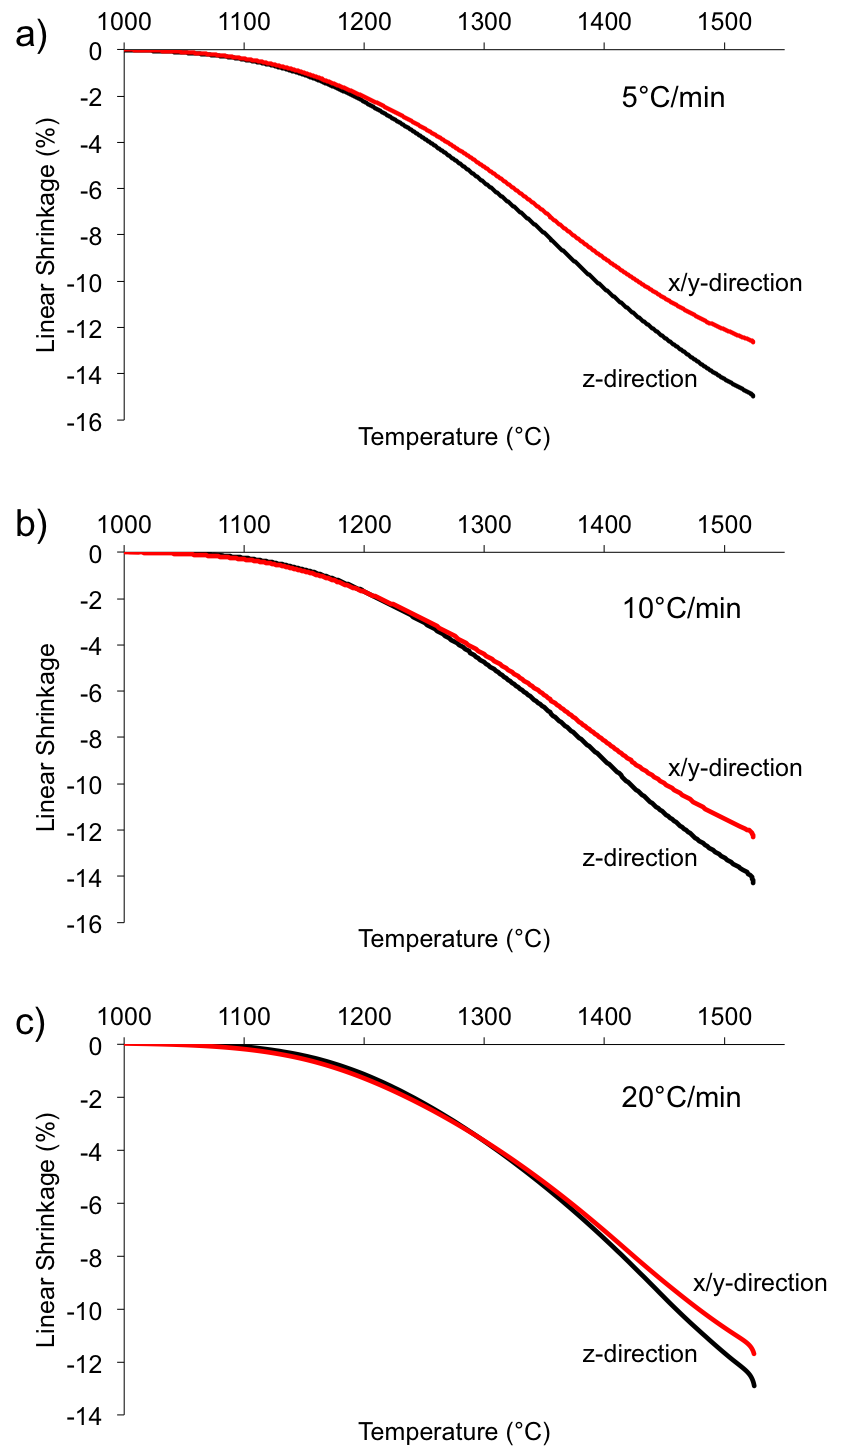
\includegraphics{Chapter-6/Figures/Figure1.png}
	\caption{Dilatometry curves of slip cast CT3000LS-SG samples heated at a) 5$^{\circ}$C/min, b) 10$^{\circ}$C/min, and c) 20$^{\circ}$C/min to 1525$^{\circ}$C measured along different directions relative to the capillary force acting during slip casting.}
	\label{Ch6-figure:Figure1}
\end{figure}
%%%

\newpage
%%%
\begin{figure}[H]
	\centering
	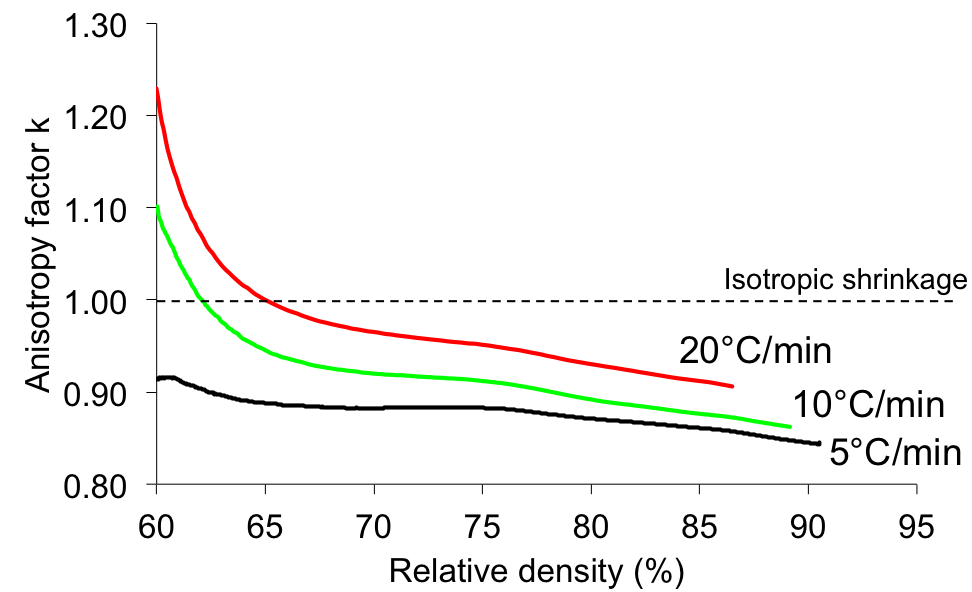
\includegraphics[width=\textwidth]{Chapter-6/Figures/Figure2.png}
	\caption{Development of the anisotropy factor for shrinkage, $k$, as a function of relative density for CT3000LS-SG samples heated at different rates.}
	\label{Ch6-figure:Figure2}
\end{figure}
%%%

\newpage
%%%
\begin{figure}[H]
	\centering
	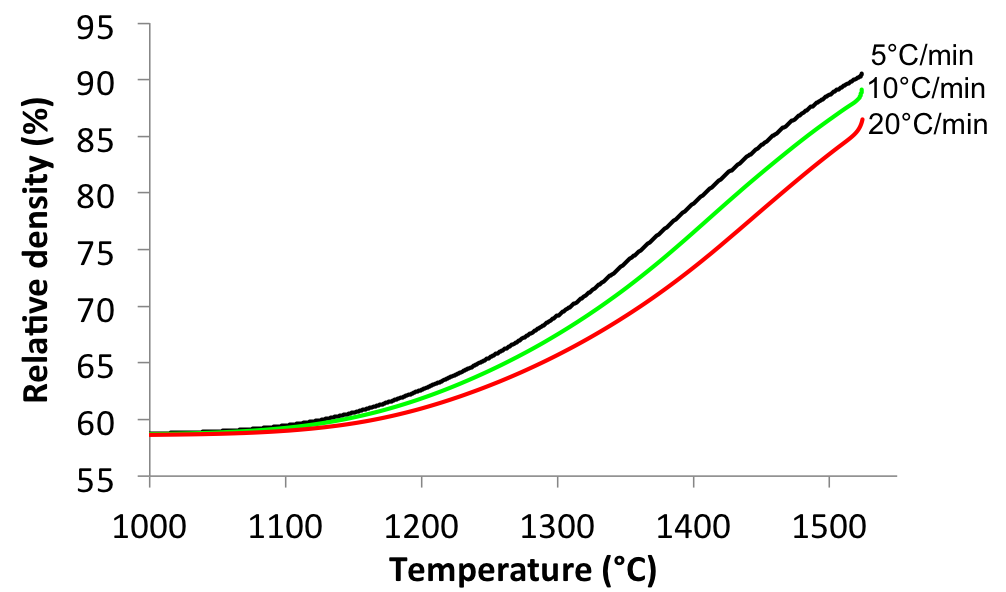
\includegraphics[width=\textwidth]{Chapter-6/Figures/Figure3.png}
	\caption{Development of the relative density corrected for anisotropy as a function of temperature for slip cast CT3000LS-SG samples for different heating rates.}
	\label{Ch6-figure:Figure3}
\end{figure}
%%%

\newpage
%%%
\begin{figure}[H]
	\centering
	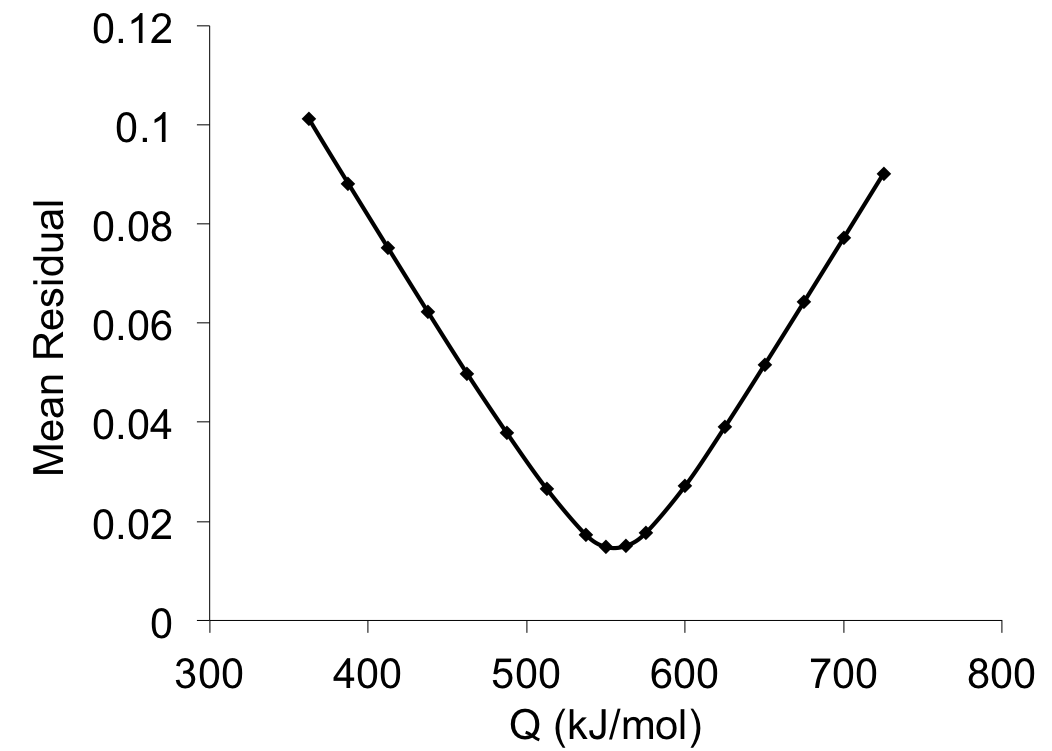
\includegraphics[width=\textwidth]{Chapter-6/Figures/Figure4.png}
	\caption{Mean residuals of the MSC curves assuming different values for the activation energy $Q$ for slip cast CT3000LS-SG samples.}
	\label{Ch6-figure:Figure4}
\end{figure}
%%%

\newpage
%%%
\begin{figure}[H]
	\centering
	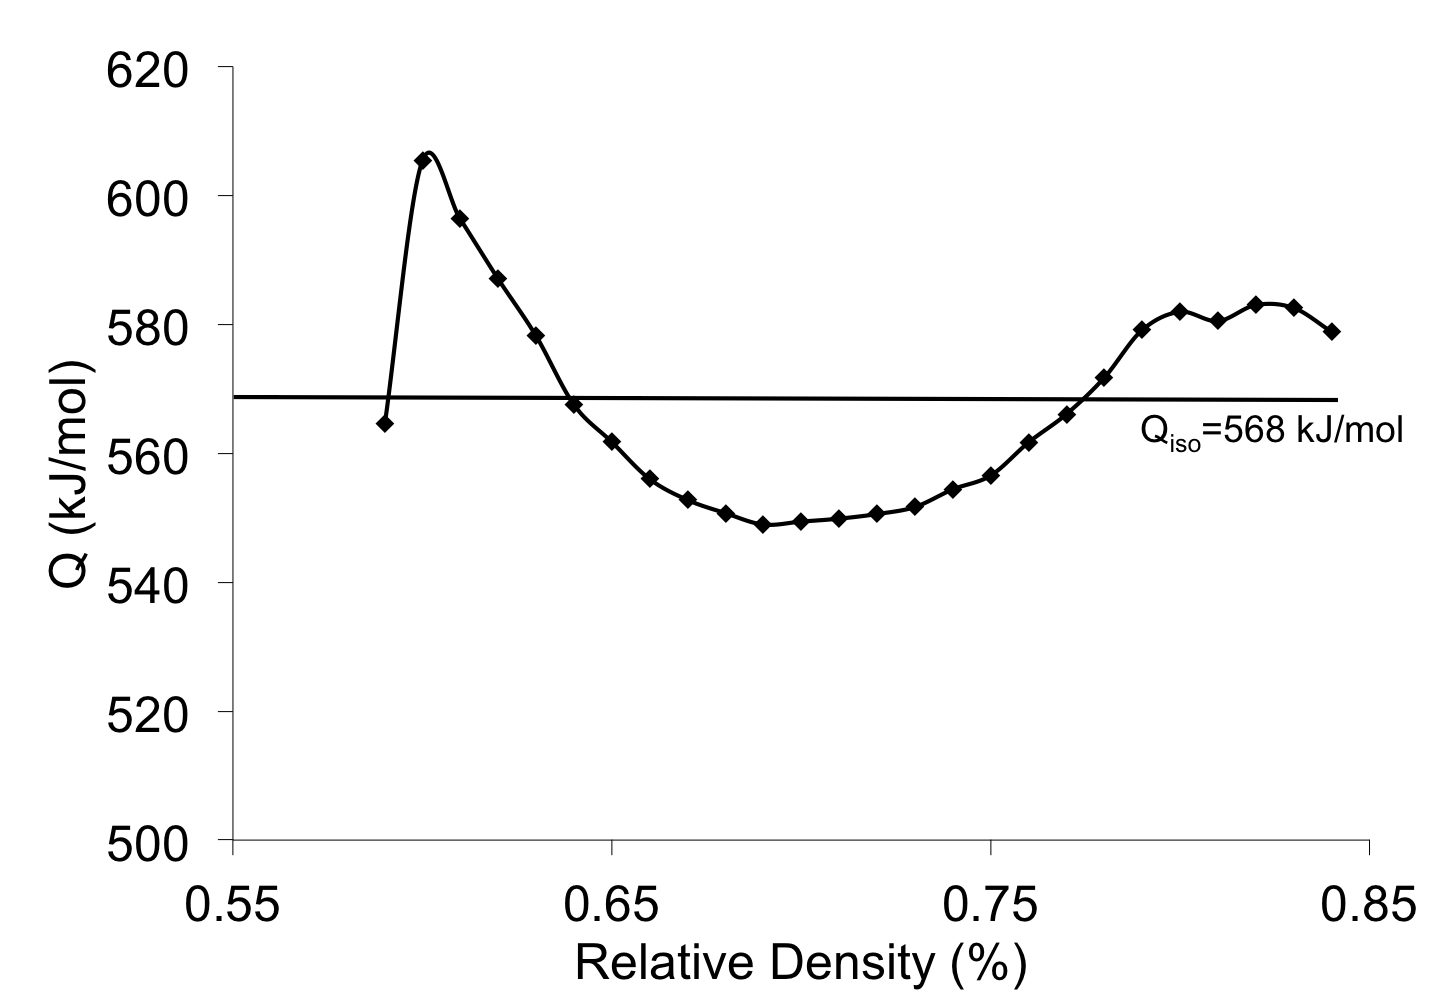
\includegraphics[width=\textwidth]{Chapter-6/Figures/Figure5.png}
	\caption{Apparent activation energy of slip cast CT3000LS-SG samples obtained from anisotropy-corrected iso-density analysis.}
	\label{Ch6-figure:Figure5}
\end{figure}
%%%

\newpage
%%%
\begin{figure}[H]
	\centering
	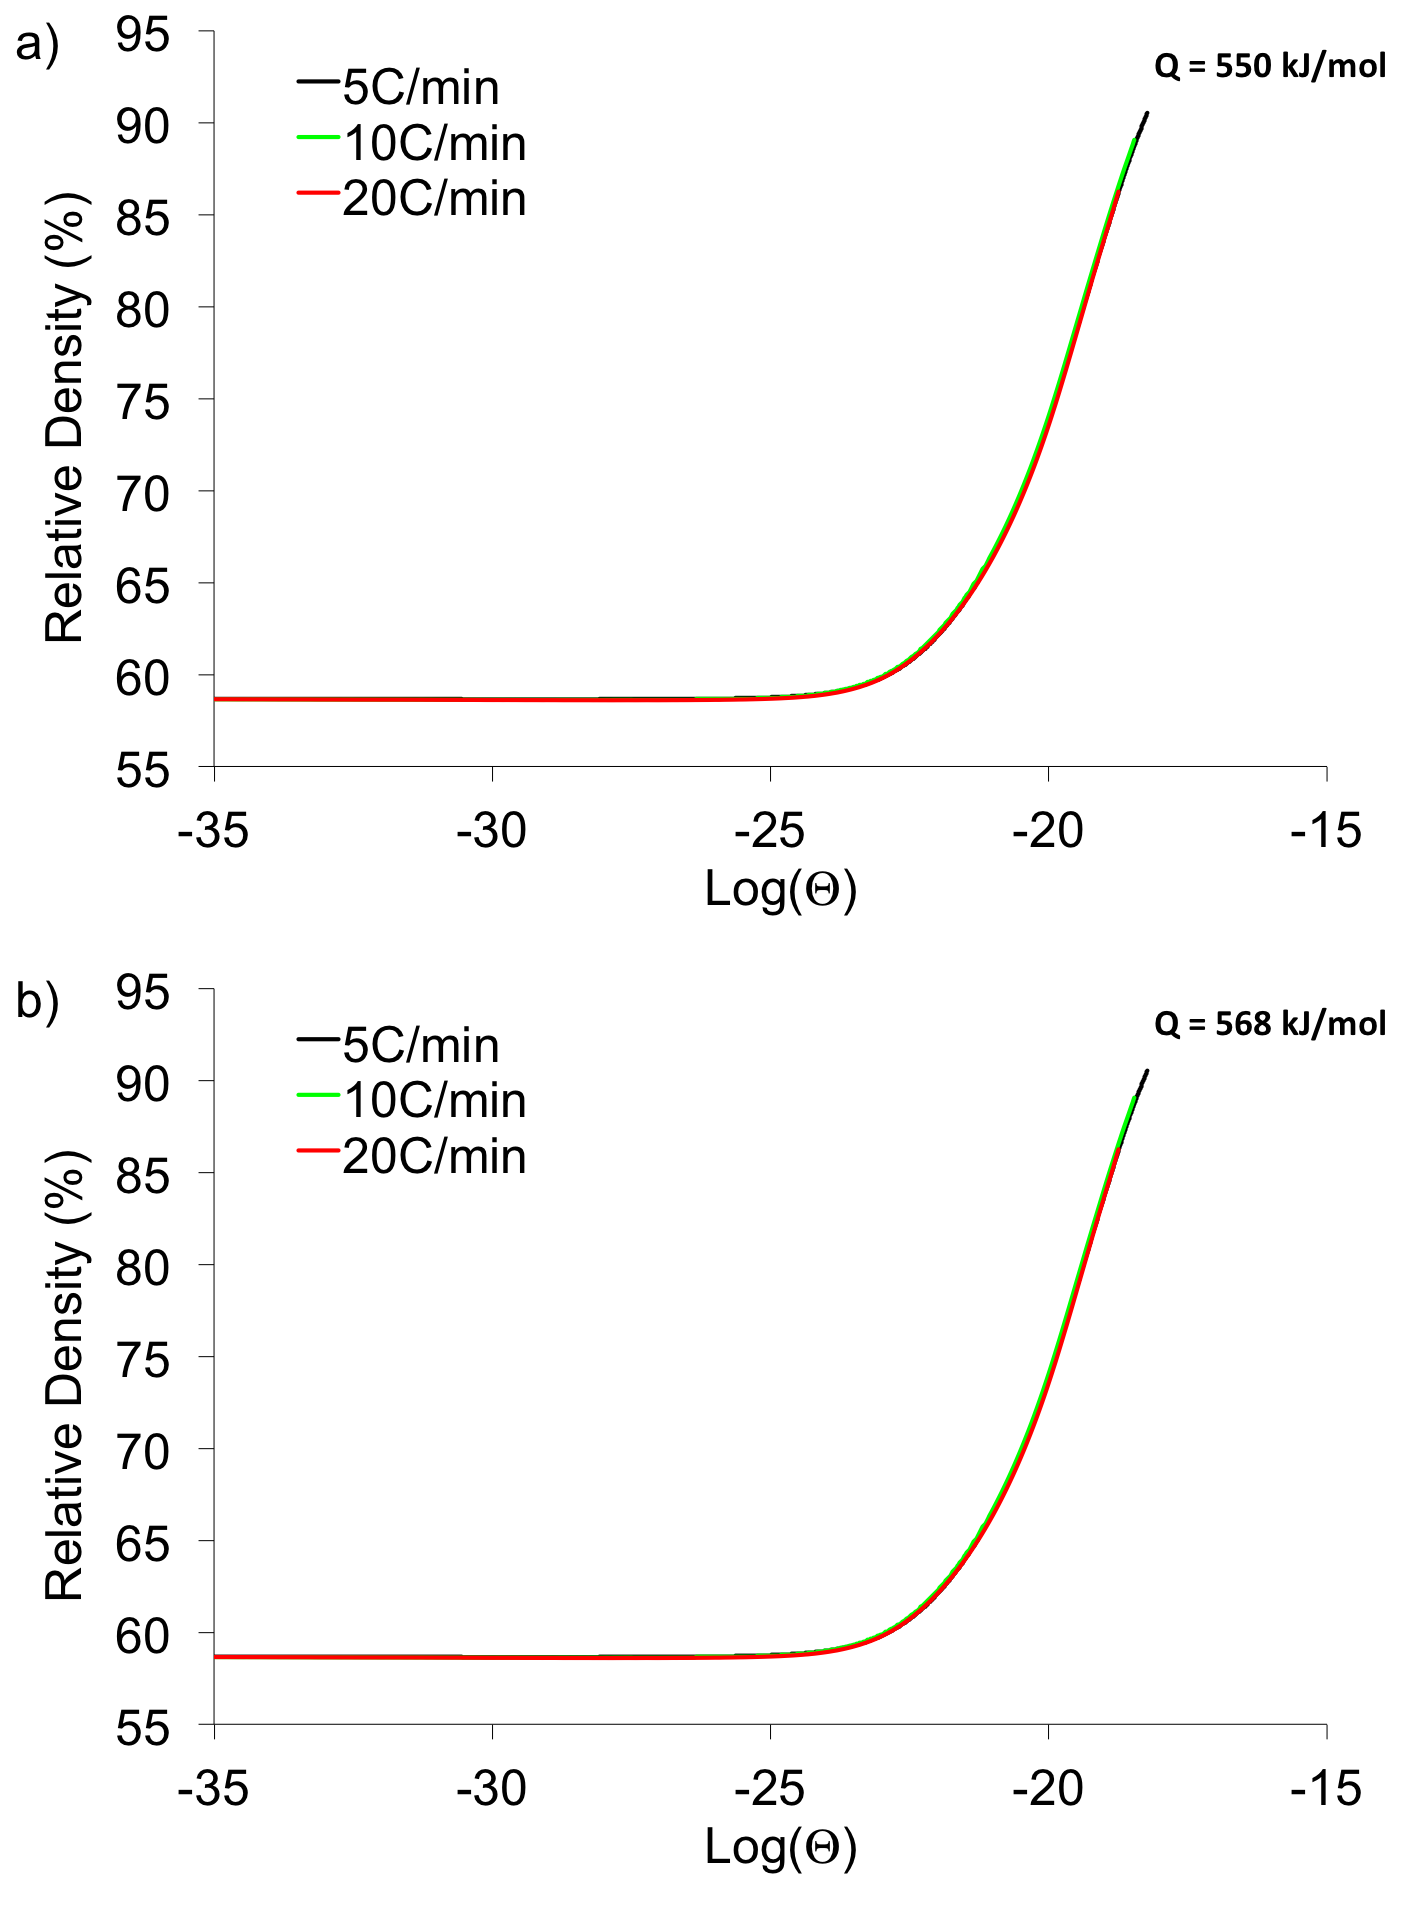
\includegraphics[width=\textwidth]{Chapter-6/Figures/Figure6.png}
	\caption{MSC curves of CT3000LS-SG samples prepared by non-aqueous slip casting using the activation energy obtained from a) minimum mean residuals, and b) the average of the iso-density analysis.}
	\label{Ch6-figure:Figure6}
\end{figure}
%%%

\newpage
%%%
\begin{figure}[H]
	\centering
	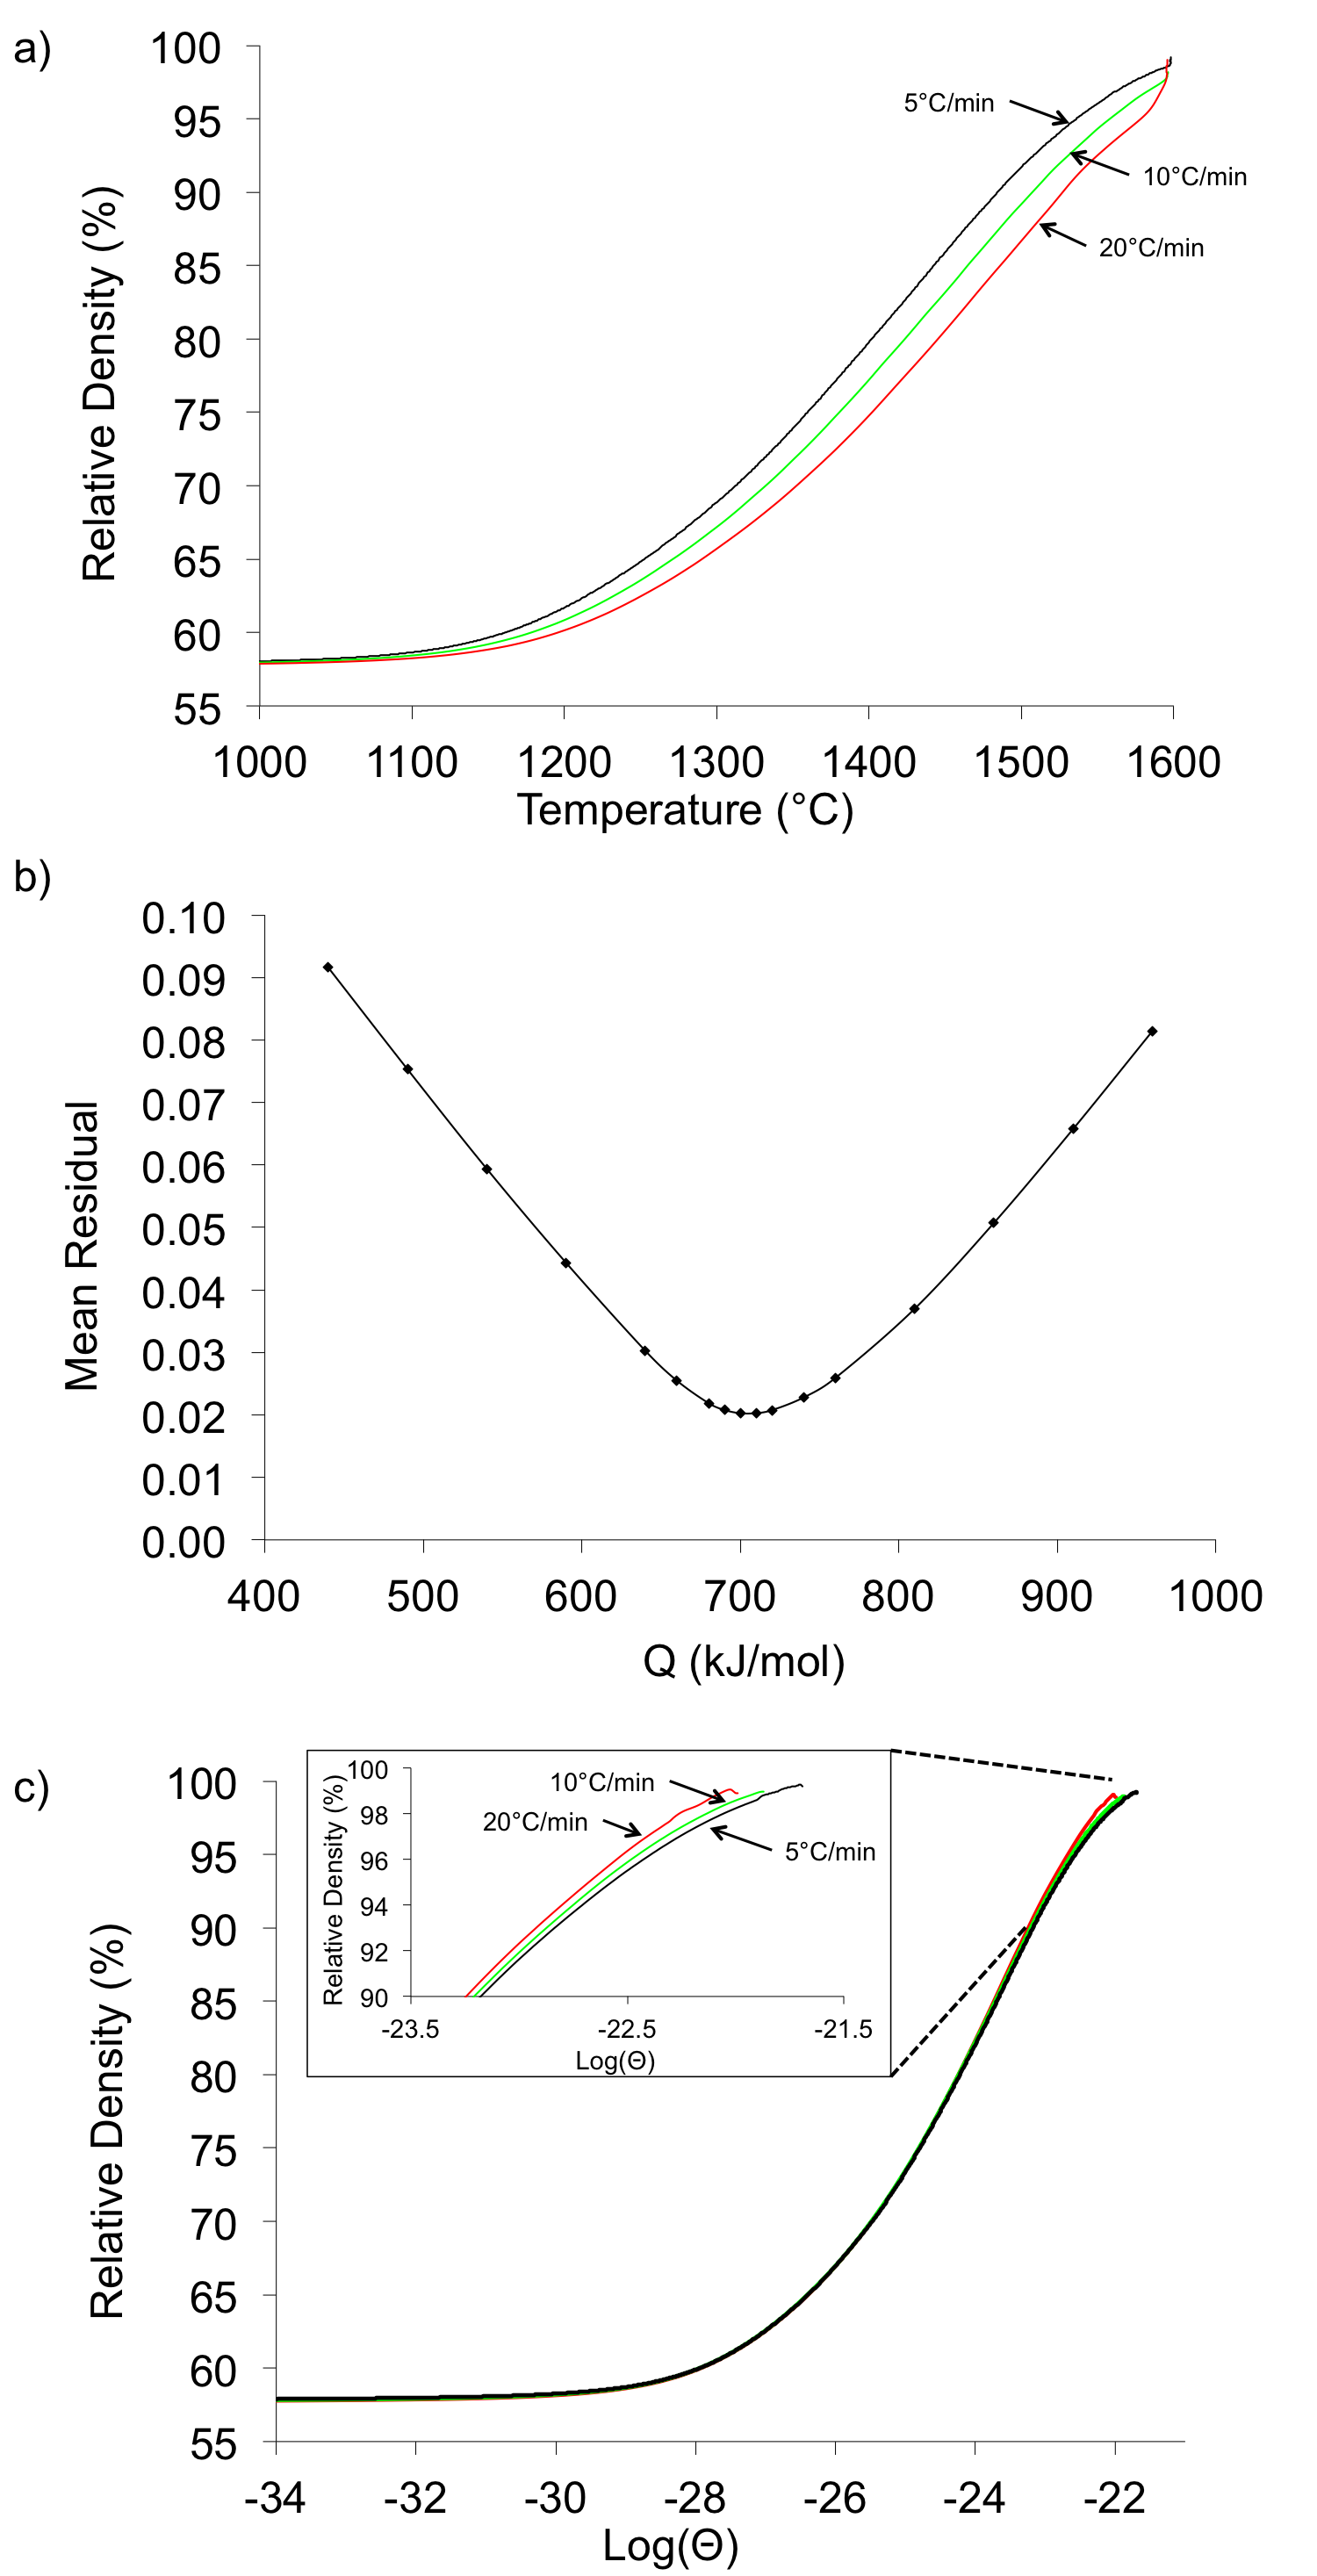
\includegraphics[width=\textwidth]{Chapter-6/Figures/Figure7.png}
	\caption{MSC curve of CT3000LS-SG samples prepared by non-aqueous slip casting neglecting the anisotropic shrinkage in the samples. $Q$ was obtained from the minimum mean residuals.}
	\label{Ch6-figure:Figure7}
\end{figure}
%%%

\newpage
%%%
\begin{figure}[H]
	\centering
	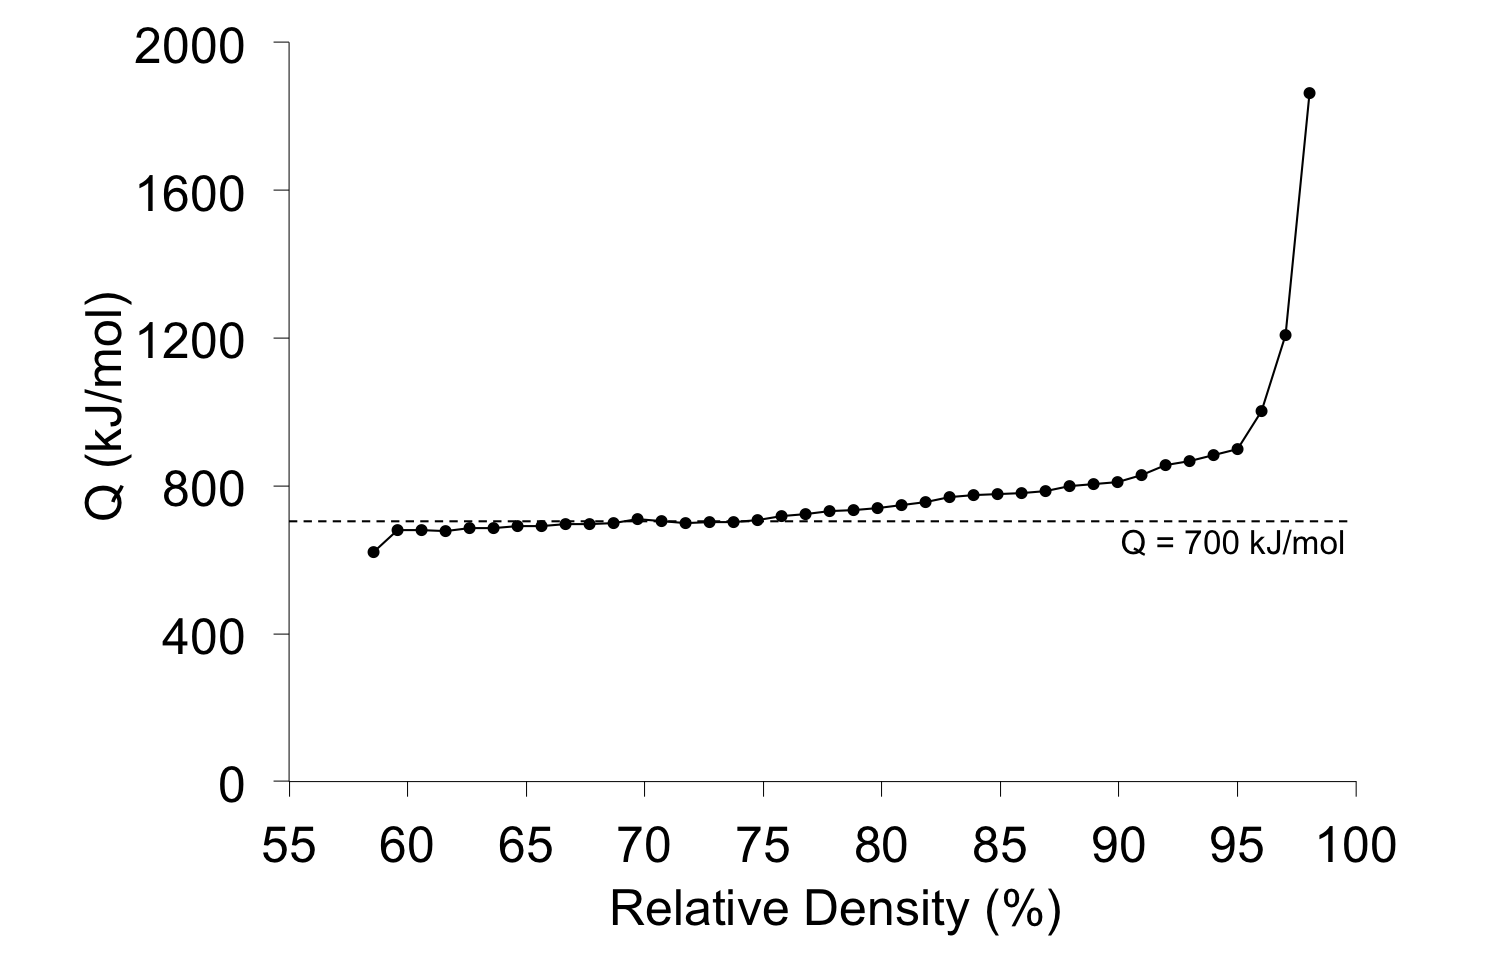
\includegraphics[width=\textwidth]{Chapter-6/Figures/Figure8.png}
	\caption{a) Densification of dry pressed CT3000LS-SG samples heated at different rates, b) mean residuals as a function of activation energy, and c) MSC for $Q$ = 700 kJ/mol obtained from the minimum mean residuals, showing divergence at densities >90\%. }
	\label{Ch6-figure:Figure8}
\end{figure}
%%%

\newpage
%%%
\begin{figure}[H]
	\centering
	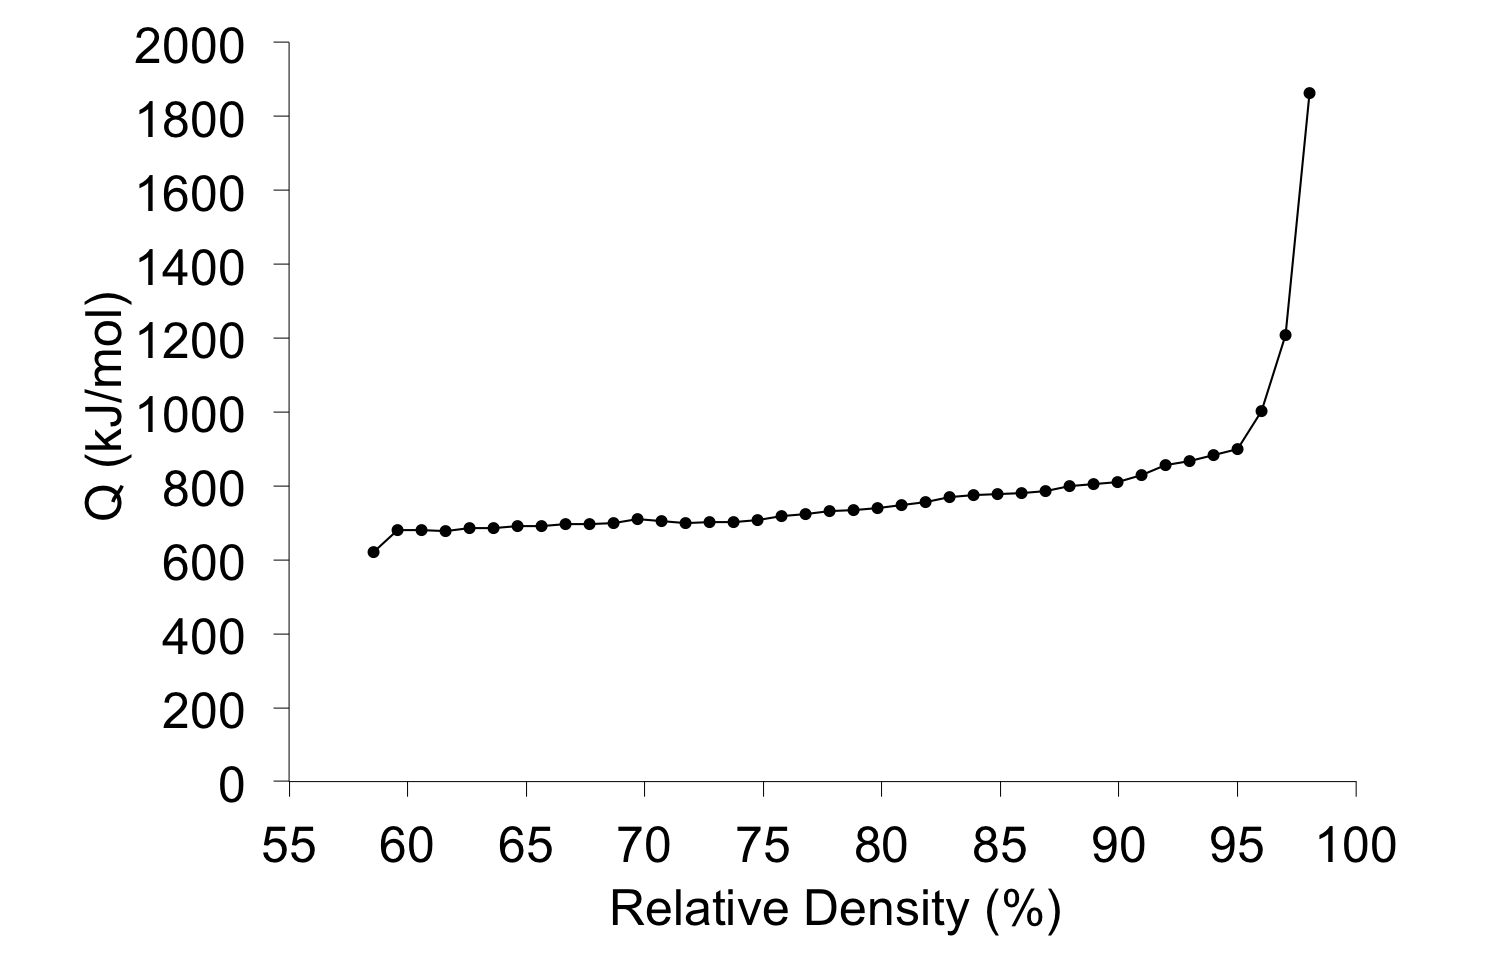
\includegraphics[width=\textwidth]{Chapter-6/Figures/Figure9.png}
	\caption{Activation energy of dry pressed CT3000LS-SG samples as a function of relative density obtained from iso-density analysis.}
	\label{Ch6-figure:Figure9}
\end{figure}
%%%

\newpage
%%%
\begin{figure}[H]
	\centering
	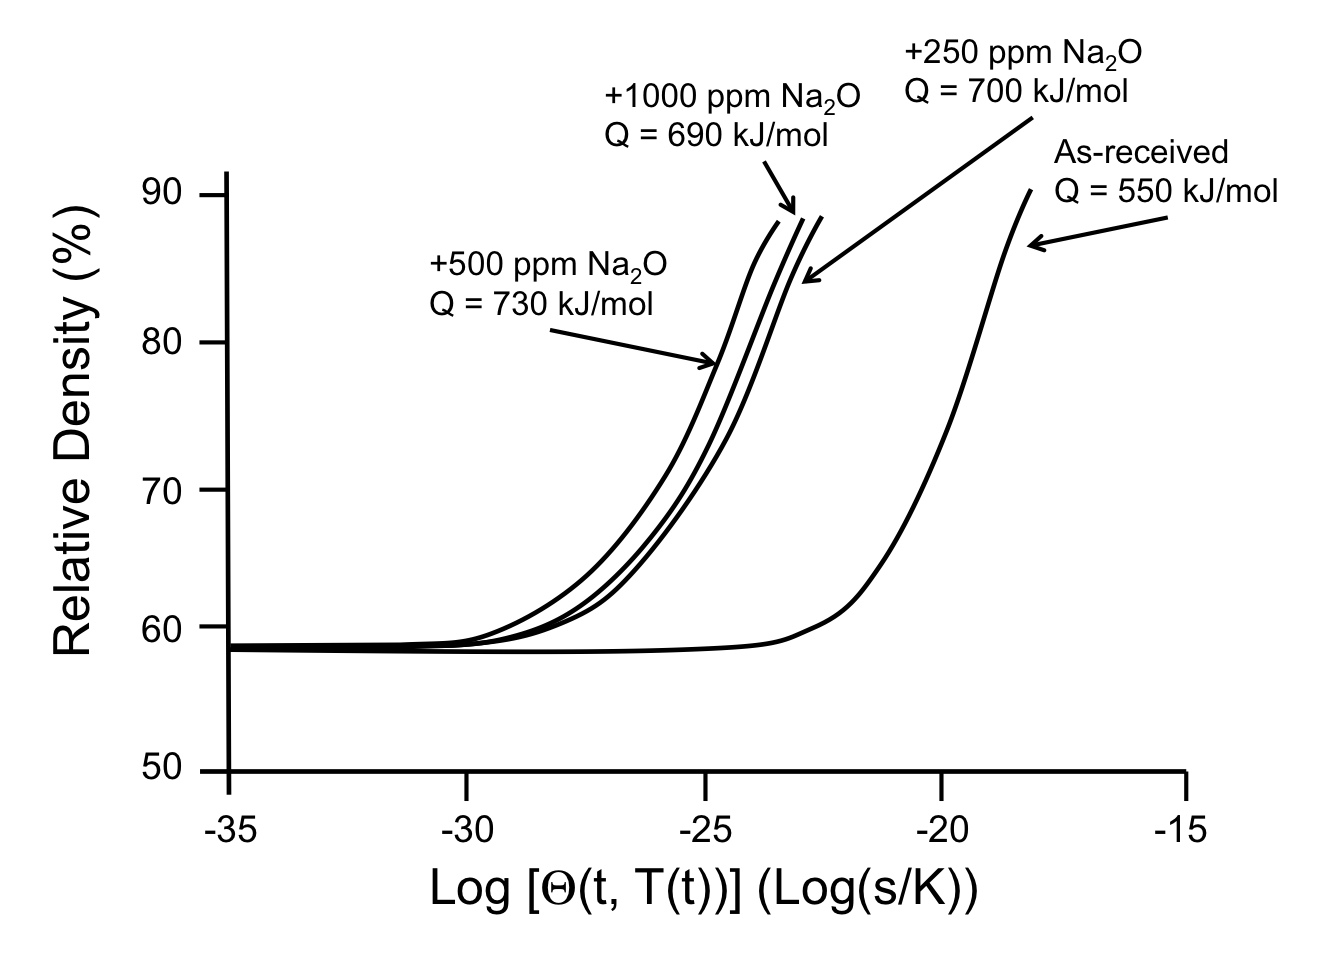
\includegraphics[width=\textwidth]{Chapter-6/Figures/Figure10.png}
	\caption{Development of the microstructural parameters, summarized in a factor $C$, as a function of relative density for a dry pressed CT3000LS-SG sample.}
	\label{Ch6-figure:Figure10}
\end{figure}
%%%

\newpage
%%%
\begin{figure}[H]
	\centering
	
\includegraphics[width=\textwidth]{Chapter-6/Figures/Figure11.png}
	\caption{MSC curves and activation energies of CT3000LS-SG samples obtained from the minimum mean residuals for samples prepared by different forming techniques.}
	\label{Ch6-figure:Figure11}
\end{figure}
%%%

\newpage
%%%
\begin{figure}[H]
	\centering
	
\includegraphics[width=\textwidth]{Chapter-6/Figures/Figure12.png}
	\caption{MSCs and activation energies for CT3000LS-SG samples prepared by non-aqueous slip casting with different Na2O concentrations.}
	\label{Ch6-figure:Figure12}
\end{figure}
%%%

\newpage
%%%
\begin{figure}[H]
	\centering
	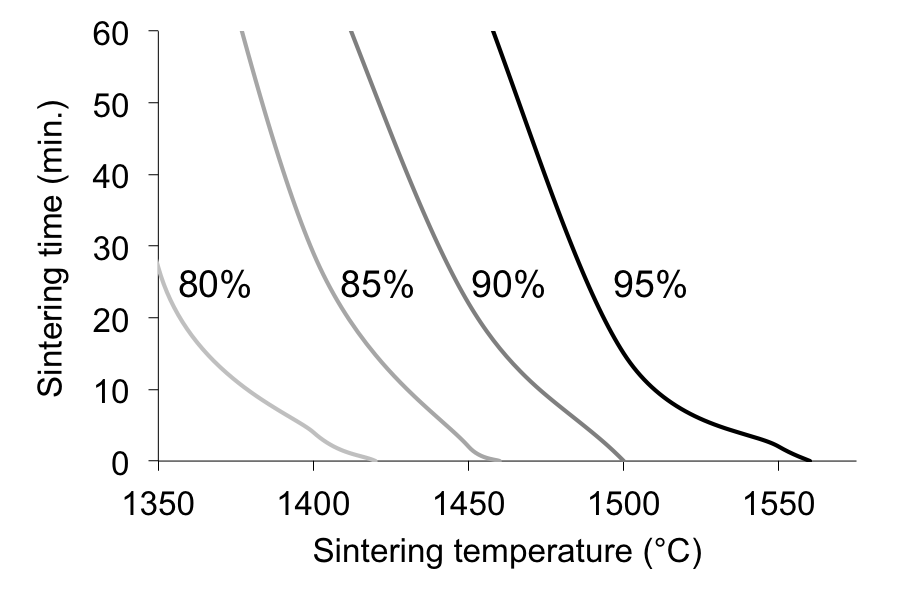
\includegraphics[width=\textwidth]{Chapter-6/Figures/Figure13.png}
	\caption{Equivalent time/temperature diagram for CT3000LS-SG samples prepared by non-aqueous slip casting heated at 10$^{\circ}$C. The contours indicate what heat treatment is required to obtain the shown density.}
	\label{Ch6-figure:Figure13}
\end{figure}
%%%

